\nopagebreak
\chapter{Objective}
\label{chap:objective}
The research proposed in this document should fulfill the project requirements set in the research proposal for workpackage B. The research should consider nonlinear extreme wave loadings. Also, the resulting data should be high fidelity and possibly lead to a reduced-order model. Lastly, it should give realistic results for expected lifetime loadings \cite{ResearchProposal2020}.
\par 
From the overview of literature shown in chapter \ref{chap:literature}, research gaps are identified. Firstly, there is a need to investigate the statistical characteristics of green water in random waves \cite{Mori2003, Chuang2018}. For complex phenomena, the use of full long-term analysis is advised for this \cite{Baarholm2010}.  Secondly, the effect of air entrapment on the green water loading is not cohesively researched, while it is known to affect experimental results \cite{Chuang2019, Greco2005}. Also, loadings due to plunging and hammer-fist type events are not well-understood, while they are known to cause the largest loadings \cite{Ariyarathne2012}. Lastly, it was found that almost all green water research has been conducted for FPSO vessels or simple geometries \cite{Chuang2019}. This means that it is difficult to predict green water loading for other types of vessels.
\par 
From the overlap of these gaps in previous research and the project objective, green water loadings on deck at the bow are chosen. 
%As stated in the proposal, the goal of WP B is to develop an extreme nonlinear wave loading model from the bottom-up. For bottom-up research a specific type of extreme nonlinear wave loading should be chosen, as this type of research attempts to understand the physics of a certain problem. 
The chosen subject should be relevant to society and there should not yet exist a way of anticipating the extreme wave loading. Green water fits this bill. Research into both the statistics and hydrodynamics of this problem will be conducted to work towards the end goal of developing a reduced-order model.

\section{Research}
\label{sec:research_topics}
The main methodology of the research will be experiments, as this is the only research tool that will give reliable data and statistics while staying affordable. 
\par 
Firstly, long running experiments will be conducted to obtain long-term data. The long-term data set will allow for identification of extreme loading events, giving more insight into the hydrodynamics of the green water problem. The data from these experiments will also be used as input for a probabilistic model, the research subject of WP C (Sanne van Essen). To do these long running experiments, the existing flume tank will be adapted. The flumetank has an inlet and outlet on each end to create a constant current. Adaptations will be made as a wedge shaped plunging wavemaker and parabolic perforated beach will be added. The flume tank including these adaptations is shown in figure \ref{fig:flumetank}. This test facility will allow for continues experiments with waves and current to be conducted. It will become a fairly unique facility with many possibilities for future research.
\begin{figure}[h]
	\centering
	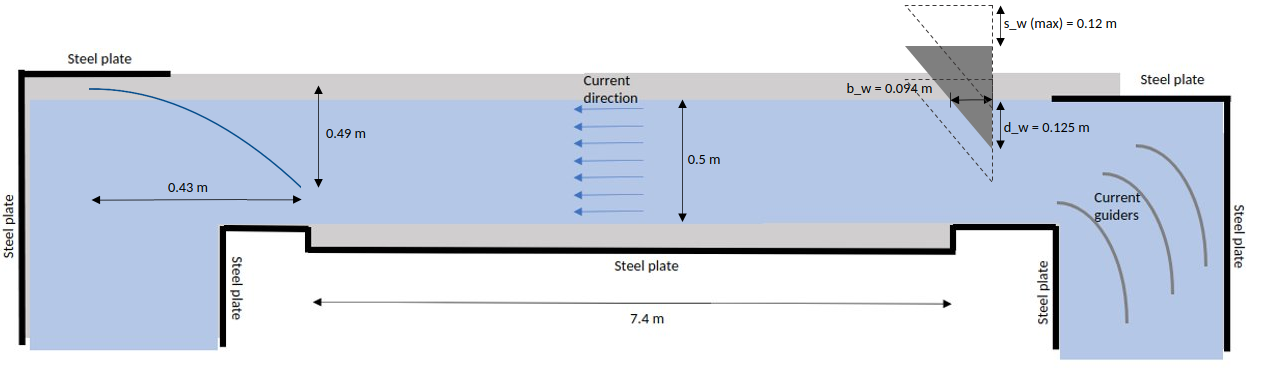
\includegraphics[width=\linewidth]{figs/FlumetankScetch.png}
	\caption{Sideview flumetank when wavemaker and beach are installed}
	\label{fig:flumetank}
\end{figure}
\par 
Scaling effects will also be researched as lack of knowledge leads to inaccurate results for green water when scaled experiments are used in research. This is problematic because scaled experiments are the main methodology of researching green water. The scaling laws are broken for air entrapment during these experiments. If we know what the influence of scaling is and how that manifests in scaled experiments, a correction can be introduced. This correction will improve the quality of experimental results, thus improving any model based on the results. To find the scaling effects, parts of the long-running experiments will be repeated at larger scales in the two towing tanks of different sizes. Because of the statistical nature of the problem, it would be beneficial to not only look at irregular waves but to also test with wave trains. This is also a good idea because of long-running experiments are not possible in the towing tanks. 
\par 
With the experimental research, data is obtained. By repeating the experiments at different scales, an indication of the fidelity of the data and what is not reliable about the data will become known. In combination with the results from the other two parts of the project, a multi-fidelity design tool will be created. The exact form this will take is dependent on the final form different parts of the project take.

\subsection{Additional research topics}
\label{sec:additional_research_topics} 
Possible additional research topics are found within the methodology. To find the lifetime loadings, long-running experiments with waves will be conducted. To achieve this the flume tank will be equipped with a wavemaker and a beach. It is an option to research the stability of the waves, the abilities of the wavemaker, or the effectiveness of the beach. 
\par
Also, data obtained from the experiments will have to be analyzed. Here, machine learning tools could be applied. From the literature study in section \ref{sec:lit_machine_learning}, it is found that they show great promise, but their use within research focused on maritime applications has been limited.
\par 
The type of green water impact (dam-break, hammer-fist or plunging) is of importance to the loading found on deck. There are also different levels of understanding for each event. From small scale experiments without forward velocities and a stationary block, the type of event that occurs is found to depend on the relative wave height at the deck and the wave steepness \cite{Greco2013}. Further improving the knowledge of when which events are expected will lead to an improvement of estimation methods for green water loading.
\par 
Almost all previous research has been conducted for FPSOs or simplified shapes. By experimentally investigating the lifetime loadings for structures not previously investigated, the understanding of the green water problem can be broadened. The applicability of previous estimation methods, possibly one from this research, on complex structures can be tested and possible improvements on the methods can be proposed.


